\chapter{Chi-squared's ditribution and related extensions}
%%%%%%%%%%%%%%%%%%%%%%%%%%%%%%%%%%%%%%%%%%%%%%
\section{Chi-squared distribution}\label{chisquared}
\subsection{Characterization}
\begin{wrapfigure}{r}{0.5\textwidth}
  \vspace{-20pt}
  \begin{center}
    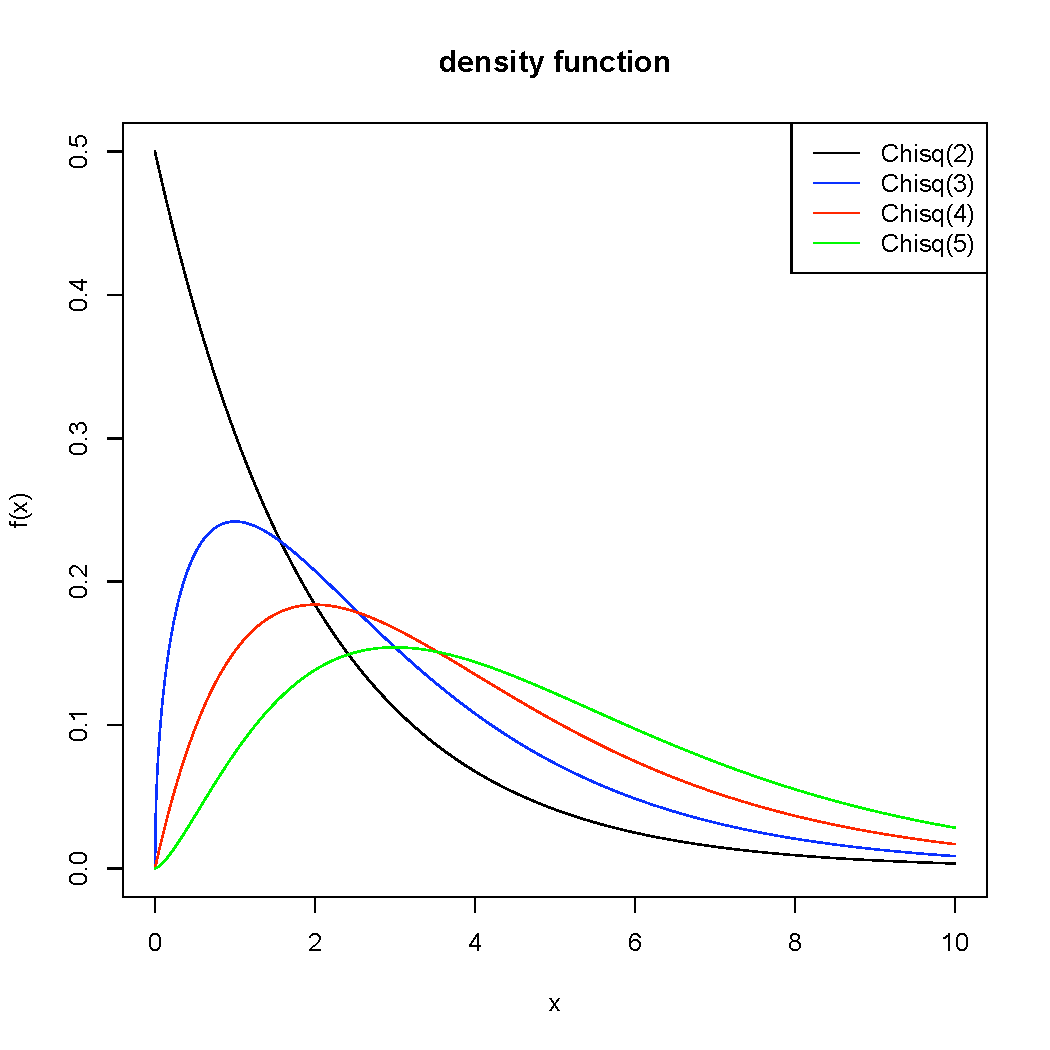
\includegraphics[width=0.48\textwidth]{img/chisqzoom}
  \end{center}
  \vspace{-20pt}  
  \caption{Density function for chi-squared distributions}
%  \vspace{-20pt}  
\end{wrapfigure}
There are many ways to define the chi-squared distribution. First, we can say a chi-squared distribution is the distribution of the sum
$$
\sum_{i=1}^k X_i^2,
$$
where $(X_i)_i$ are i.i.d. normally distributed $\mcal N(0,1)$ and a given $k$. In this context, $k$ is assumed to be an integer.

We can also define the chi-squared distribution by its density, which is
$$
f(x) = \frac{x^{\frac{k}{2}-1}}{\Gamma(\frac{k}{2}) 2^{\frac{k}{2}} }  e^{-\frac{x}{2} },  
$$
where $k$ is the so-called degrees of freedom and $x\geq 0$. One can notice that is the density of a gamma distribution $\mcal G(\frac{k}{2},\frac{1}{2})$, so $k$ is not necessarily an integer. Thus the distribution function can be expressed with the incomplete gamma function
$$
F(x) = \frac{\gamma(\frac{k}{2},\frac{x}{2})}{\Gamma(\frac{k}{2})}. 
$$

Thirdly, the chi-squared distribution can be defined in terms of its moment generating function
$$
M(t) = (1-2t)^{-\frac{k}{2}},
$$
or its characteristic function
$$
\phi(t) =(1-2it)^{-\frac{k}{2}}.
$$ 

\subsection{Properties}
The expectation and the variance of the chi-squared distribution are simply
$E(X) = k $ and $Var(X)=2k$. Raw moments are given by
$$
E(X^r) =\left(\frac{1}{2}\right)^r\frac{\Gamma(\frac{k}{2}+r)}{\Gamma(\frac{k}{2})}.
$$


\subsection{Estimation}
Same as gamma distribution ??

\subsection{Random generation}
For an integer $k$, just sum the square of $k$ normal variable. Otherwise use the algorithm for the gamma distribution.

\subsection{Applications}
The chi-squared distribution is widely used for inference, typically as pivotal function.

%%%%%%%%%%%%%%%%%%%%%%%%%%%%%%%%%%%%%%%%%%%%%%%%%
\newpage
\section{Chi distribution}
\subsection{Characterization}
\begin{wrapfigure}{r}{0.5\textwidth}
  \vspace{-20pt}
  \begin{center}
    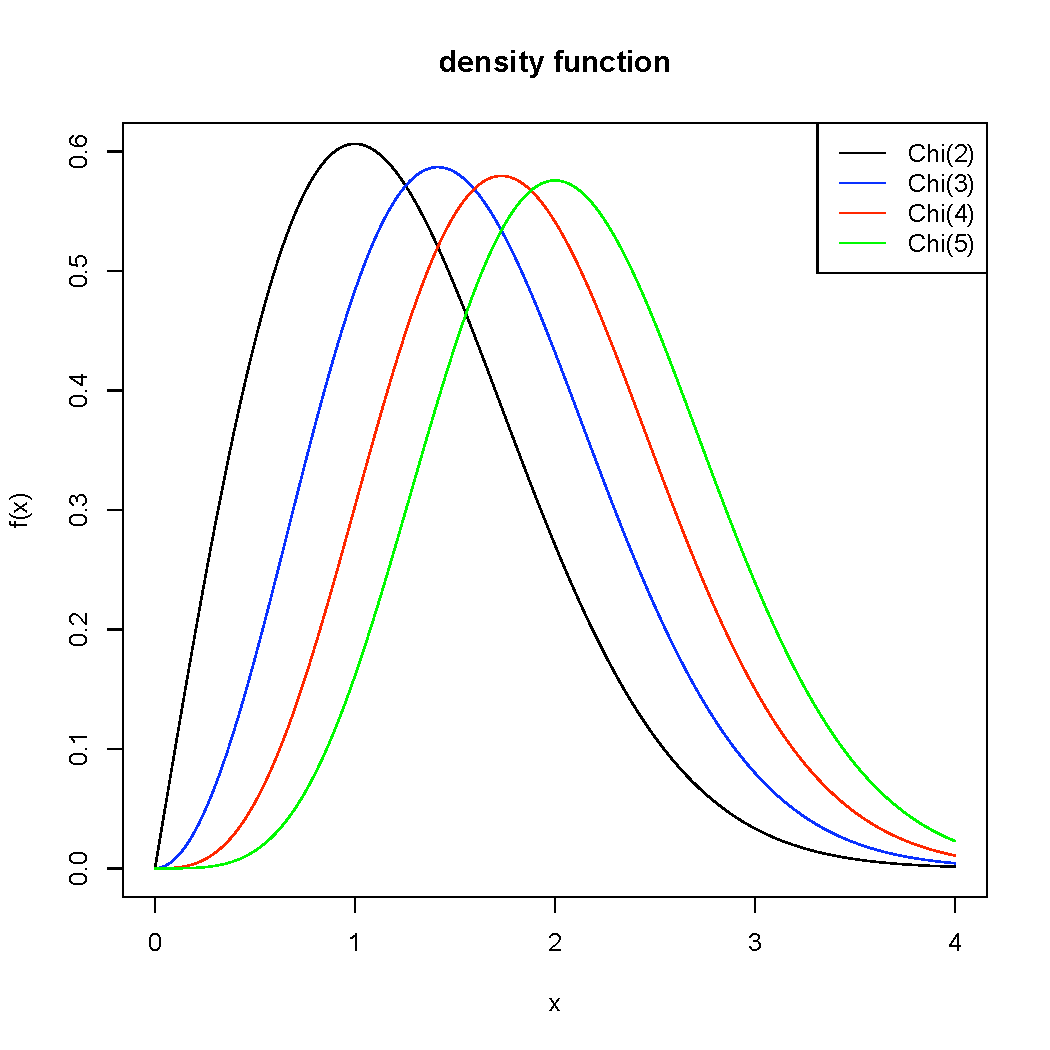
\includegraphics[width=0.48\textwidth]{img/chizoom}
  \end{center}
  \vspace{-20pt}  
  \caption{Density function for chi distributions}
%  \vspace{-20pt}  
\end{wrapfigure}
This is the distribution of the sum
$$
\sqrt{\sum_{i=1}^k X_i^2},
$$
where $(X_i)_i$ are i.i.d. normally distributed $\mcal N(0,1)$ and a given $k$. This is equivalent as the distribution of a square root of a chi-squared distribution (hence the name). 

The density function has a closed form
$$
f(x) = \frac{x^{k-1}}{2^{\frac{k}{2}-1}\Gamma\left(\frac{k}{2}\right)} e^{-\frac{x^2}{2}},
$$
where $x>0$.
The distribution function can be expressed in terms of the gamma incomplete function
$$
F(x) = \frac{\gamma(\frac{k}{2}, \frac{x^2}{2})}{\Gamma\left(\frac{k}{2}\right)},
$$
for $x>0$. 

Characteristic function and moment generating function exist and are expressed by
$$
\phi(t) = {\,}_1F_1\left(\frac{k}{2},\frac{1}{2},\frac{-t^2}{2}\right)+it\sqrt{2}\frac{\Gamma\left(\frac{k+1}{2}\right)}{\Gamma\left(\frac{k}{2}\right)} 
$$
and
$$
M(t) = {\,}_1F_1\left(\frac{k}{2},\frac{1}{2},\frac{t^2}{2}\right) +t\sqrt{2}\frac{\Gamma\left(\frac{k+1}{2}\right)}{\Gamma\left(\frac{k}{2}\right)}.
$$


\subsection{Properties}
The expectation and the variance of a chi distribution are given by $E(X) =\frac{\sqrt{2} \Gamma(\frac{k+1}{2})}{ \Gamma(\frac{k}{2})} $ and $Var(X) = k-E^2(X)$. Other moments are given by
$$
E(X^r) = 2^{\frac{r}{2}}\frac{ \Gamma(\frac{k+r}{2})}{ \Gamma(\frac{k}{2})},
$$
for $k+r>0$.

\subsection{Estimation}
The maximum likelihood estimator of $k$ satisfies the following equation
$$
\frac{1}{2}\psi\left(\frac{k}{2}\right)+ \frac{\log(2)}{2} = \frac{1}{n}\sum_{i=1}^n\log(X_i),
$$
where $\psi$ denotes the digamma function. This equation can be solved on the positive real line or just the set of positive integers.

\subsection{Random generation}
Take the square root of a chi-squared random variable.

\subsection{Applications}
NEED REFERENCE

%%%%%%%%%%%%%%%%%%%%%%%%%%%%%%%%%%%%%%%%%%%%%%%%%%%%
\section{Non central chi-squared distribution}

\subsection{Characterization}
\begin{wrapfigure}{r}{0.5\textwidth}
  \vspace{-20pt}
  \begin{center}
    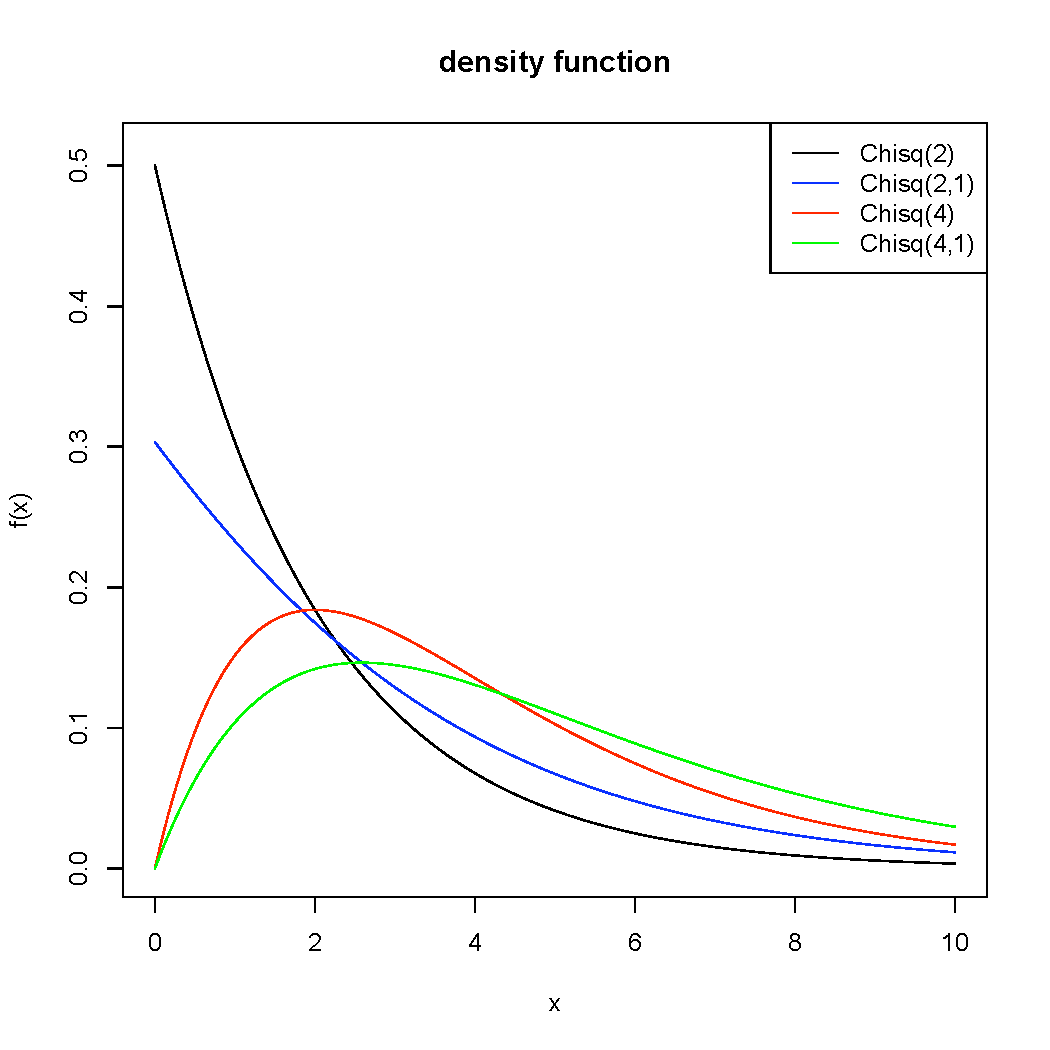
\includegraphics[width=0.48\textwidth]{img/noncentrchisqzoom}
  \end{center}
  \vspace{-20pt}  
  \caption{Density function for non central chi-squared distributions}
%  \vspace{-20pt}  
\end{wrapfigure}
The non central chi-squared distribution is the distribution of the sum
$$
\sum_{i=1}^k X_i^2,
$$
where $(X_i)_i$ are independent normally distributed $\mcal N(\mu_i,1)$, 
i.e. non centered normal random variable. We generally define the non central
chi-squared distribution by the density
$$
f(x) =  \frac{1}{2} \left(\frac{x}{\lambda}\right)^{\frac{k-2}{4}}  e^{-\frac{x+\lambda}{2} } I_{\frac{k}{2}-1} \left(\sqrt{\lambda x}\right) ,
$$
for $x>0$, $k\geq 2$ the degree of freedom, $\lambda$ the non central parameter and $I_\lambda$ the Bessel's modified function. $\lambda$ is related to the previous sum by 
$$
\lambda = \sum_{i=1}^k \mu_i^2.
$$

The distribution function can be expressed in terms of a serie
$$
F(x) = \sum_{j=0}^{+\infty} e^{\frac{-\lambda}{2}} \frac{(\frac{\lambda}{2})^j \gamma(j+\frac{k}{2},\frac{x}{2})}{j!\Gamma(j+\frac{k}{2})} ,
$$
for $x>0$ where $\gamma(.,.)$ denotes the incomplete gamma function.

Moment generating function for the non central chi-squared distribution exists
$$
M(t) = \frac{e^{\frac{\lambda  t}{1-2t}}}{(1-2t)^{\frac{k}{2}}}
$$
and the characteristic function
$$
\phi(t) = \frac{e^{\frac{\lambda i t}{1-2it}}}{(1-2it)^{\frac{k}{2}}},
$$
from which we see it is a convolution of a gamma distribution and a compound Poisson distribution.

\subsection{Properties}
Moments for the non central chi-squared distribution are given by
$$
E(X^n) = 2^{n-1}(n-1)!(k+n\lambda)+\sum_{j=1}^{n-1} \frac{(n-1)!2^{j-1}}{(n-j)!}(k+j\lambda )E(X^{n-j}),
$$
where the first raw moment is
$$
E(X) = k+\lambda. 
$$
The variance is $Var(X) = 2(k+2\lambda)$.


\subsection{Estimation}
\cite{liyu} and \cite{saxena}

\subsection{Random generation}
For integer $k$ degrees of freedom, we can use the definition of the sum, i.e. sum $k$ idependent normal random variables $\mcal N(\sqrt{\frac{\lambda}{k}},1)$.

\subsection{Applications}
NEED REFERENCE

%%%%%%%%%%%%%%%%%%%%%%%%%%%%%%%%%%%%%%%%%%
\section{Non central chi distribution}
\subsection{Characterization}

This is the distribution of the sum
$$
\sqrt{\sum_{i=1}^k X_i^2},
$$
where $(X_i)_i$ are i.i.d. normally distributed $\mcal N(\mu_i,1)$ and a given $k$. This is equivalent as the distribution of a square root of a non central chi-squared distribution (hence the name). 

We generally define the non central chi distribution by
$$
f(x) = \frac{\lambda x^{k}}{(\lambda x)^{\frac{k}{2}} } e^{-\frac{x^2+\lambda^2}{2}} I_{\frac{k}{2}-1}(\lambda x),
$$
where $x>0$ and $I_.(.)$ denotes the modified Bessel's function.
The distribution function can be expressed in terms of the gamma incomplete function
$$
F(x) = ??,
$$
for $x>0$. 




\subsection{Properties}
The expectation and the variance of a chi distribution are given by $$
E(X) =\sqrt{\frac{\pi}{2}}L_{1/2}^{(k/2-1)}\left(\frac{-\lambda^2}{2}\right)
$$ and $$
Var(X) = k+\lambda^2-E^2(X), $$
where $L_.^{(.)}$ denotes the generalized Laguerre polynomials.
Other moments are given by
$$
E(X^r) = ??,
$$
for $k+r>0$.

\subsection{Estimation}
NEED REFERENCE

\subsection{Random generation}
NEED REFERENCE

\subsection{Applications}
NEED REFERENCE

%%%%%%%%%%%%%%%%%%%%%%%%%%%%%%%%%%%%%%%%%%%%%%%
\section{Inverse chi-squared distribution}
\begin{wrapfigure}{r}{0.5\textwidth}
  \vspace{-20pt}
  \begin{center}
    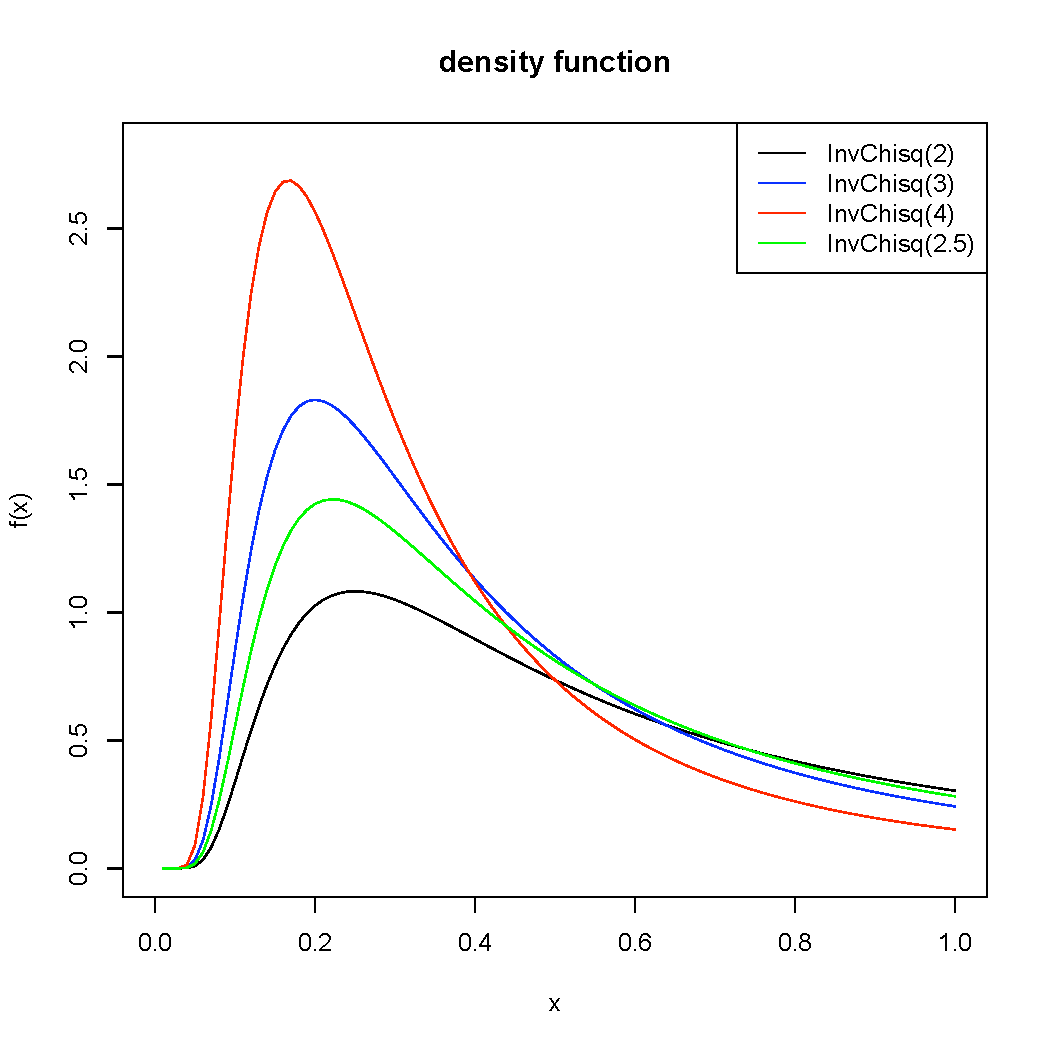
\includegraphics[width=0.48\textwidth]{img/invchisqzoom}
  \end{center}
  \vspace{-20pt}  
  \caption{Density function for inverse chi-squared distributions}
%  \vspace{-20pt}  
\end{wrapfigure}
The inverse chi-squared distribution is simply the distribution of $\frac{1}{X}$ when $X$ is chi-squared distributed.
We can also define the chi-squared distribution by its density, which is
$$
f(x) = \frac{2^{-\frac{k}{2}}}{\Gamma(\frac{k}{2})}\,x^{-\frac{k-2}{2}}  e^{-\frac{1}{2x}},
$$
where $k$ is the so-called degrees of freedom and $x\geq 0$. Thus the distribution function can be expressed with the incomplete gamma function
$$
F(x) = \frac{\Gamma(\frac{k}{2},\frac{1}{2x})}{\Gamma(\frac{k}{2})},
$$
where $\Gamma(.,.)$ the upper incomplete gamma function.

Thirdly, the chi-squared distribution can be defined in terms of its moment generating function
$$
M(t) = \frac{2}{\Gamma(\frac{k}{2})} \left(\frac{-t}{2}\right)^{\!\!\frac{k}{4}} K_{\frac{k}{2}}\!\left(\sqrt{-2t}\right),
$$
or its characteristic function
$$
\phi(t) =\frac{2}{\Gamma(\frac{k}{2})} \left(\frac{-it}{2}\right)^{\!\!\frac{k}{4}} K_{\frac{k}{2}}\!\left(\sqrt{-2it}\right).
$$ 

\subsection{Properties}
The expectation and the variance of the chi-squared distribution are simply
$E(X) = \frac{1}{k-2} $ if $k>2$ and $Var(X)=\frac{2}{(k-2)^2(k-4)}$. Raw moments are given by
$$
E(X^r) =??
$$


\subsection{Estimation}
Maximum likelihood estimator for $k$ verifies the equation
$$
\psi\left(\frac{k}{2}\right) = -\log(2)-\frac{1}{n}\sum_{i=1}^n \log(x_i),
$$
where $\psi$ denotes the digamma function.

\subsection{Random generation}
Simply inverse a chi-squared random variable

\subsection{Applications}
NEED REFERENCE

%%%%%%%%%%%%%%%%%%%%%%%%%%%%%%%%%%%%%%%%%%%%%
\section{Scaled inverse chi-squared distribution}
\subsection{Characterization}
TODO
\subsection{Properties}
TODO
\subsection{Estimation}
TODO
\subsection{Random generation}
TODO
\subsection{Applications}
TODO
